\nexthint{Example - slide stm. abstract}
\begin{frame}{Relational verification in practice}
  \begin{block}{REFINITY}
    \begin{itemize}
      \setlength\itemsep{0.5\itemsep}
    \item Built on top of the KeY automated theorem prover
    \item Enables relational verification of ``Java'' with placeholders
    \item Placeholders are subject to Abstract Execution
    \item Has been sufficiently powerful to verify statement level refactorings\footnote{See Dominic Steinhöfel's PhD thesis: \href{Abstract Execution}{https://tuprints.ulb.tu-darmstadt.de/8540/}}
    \end{itemize}
  \end{block}
\end{frame}

\nexthint{Example - slide stm. abs. proved}
\begin{frame}\vspace*{-5mm}
  \begin{center}
    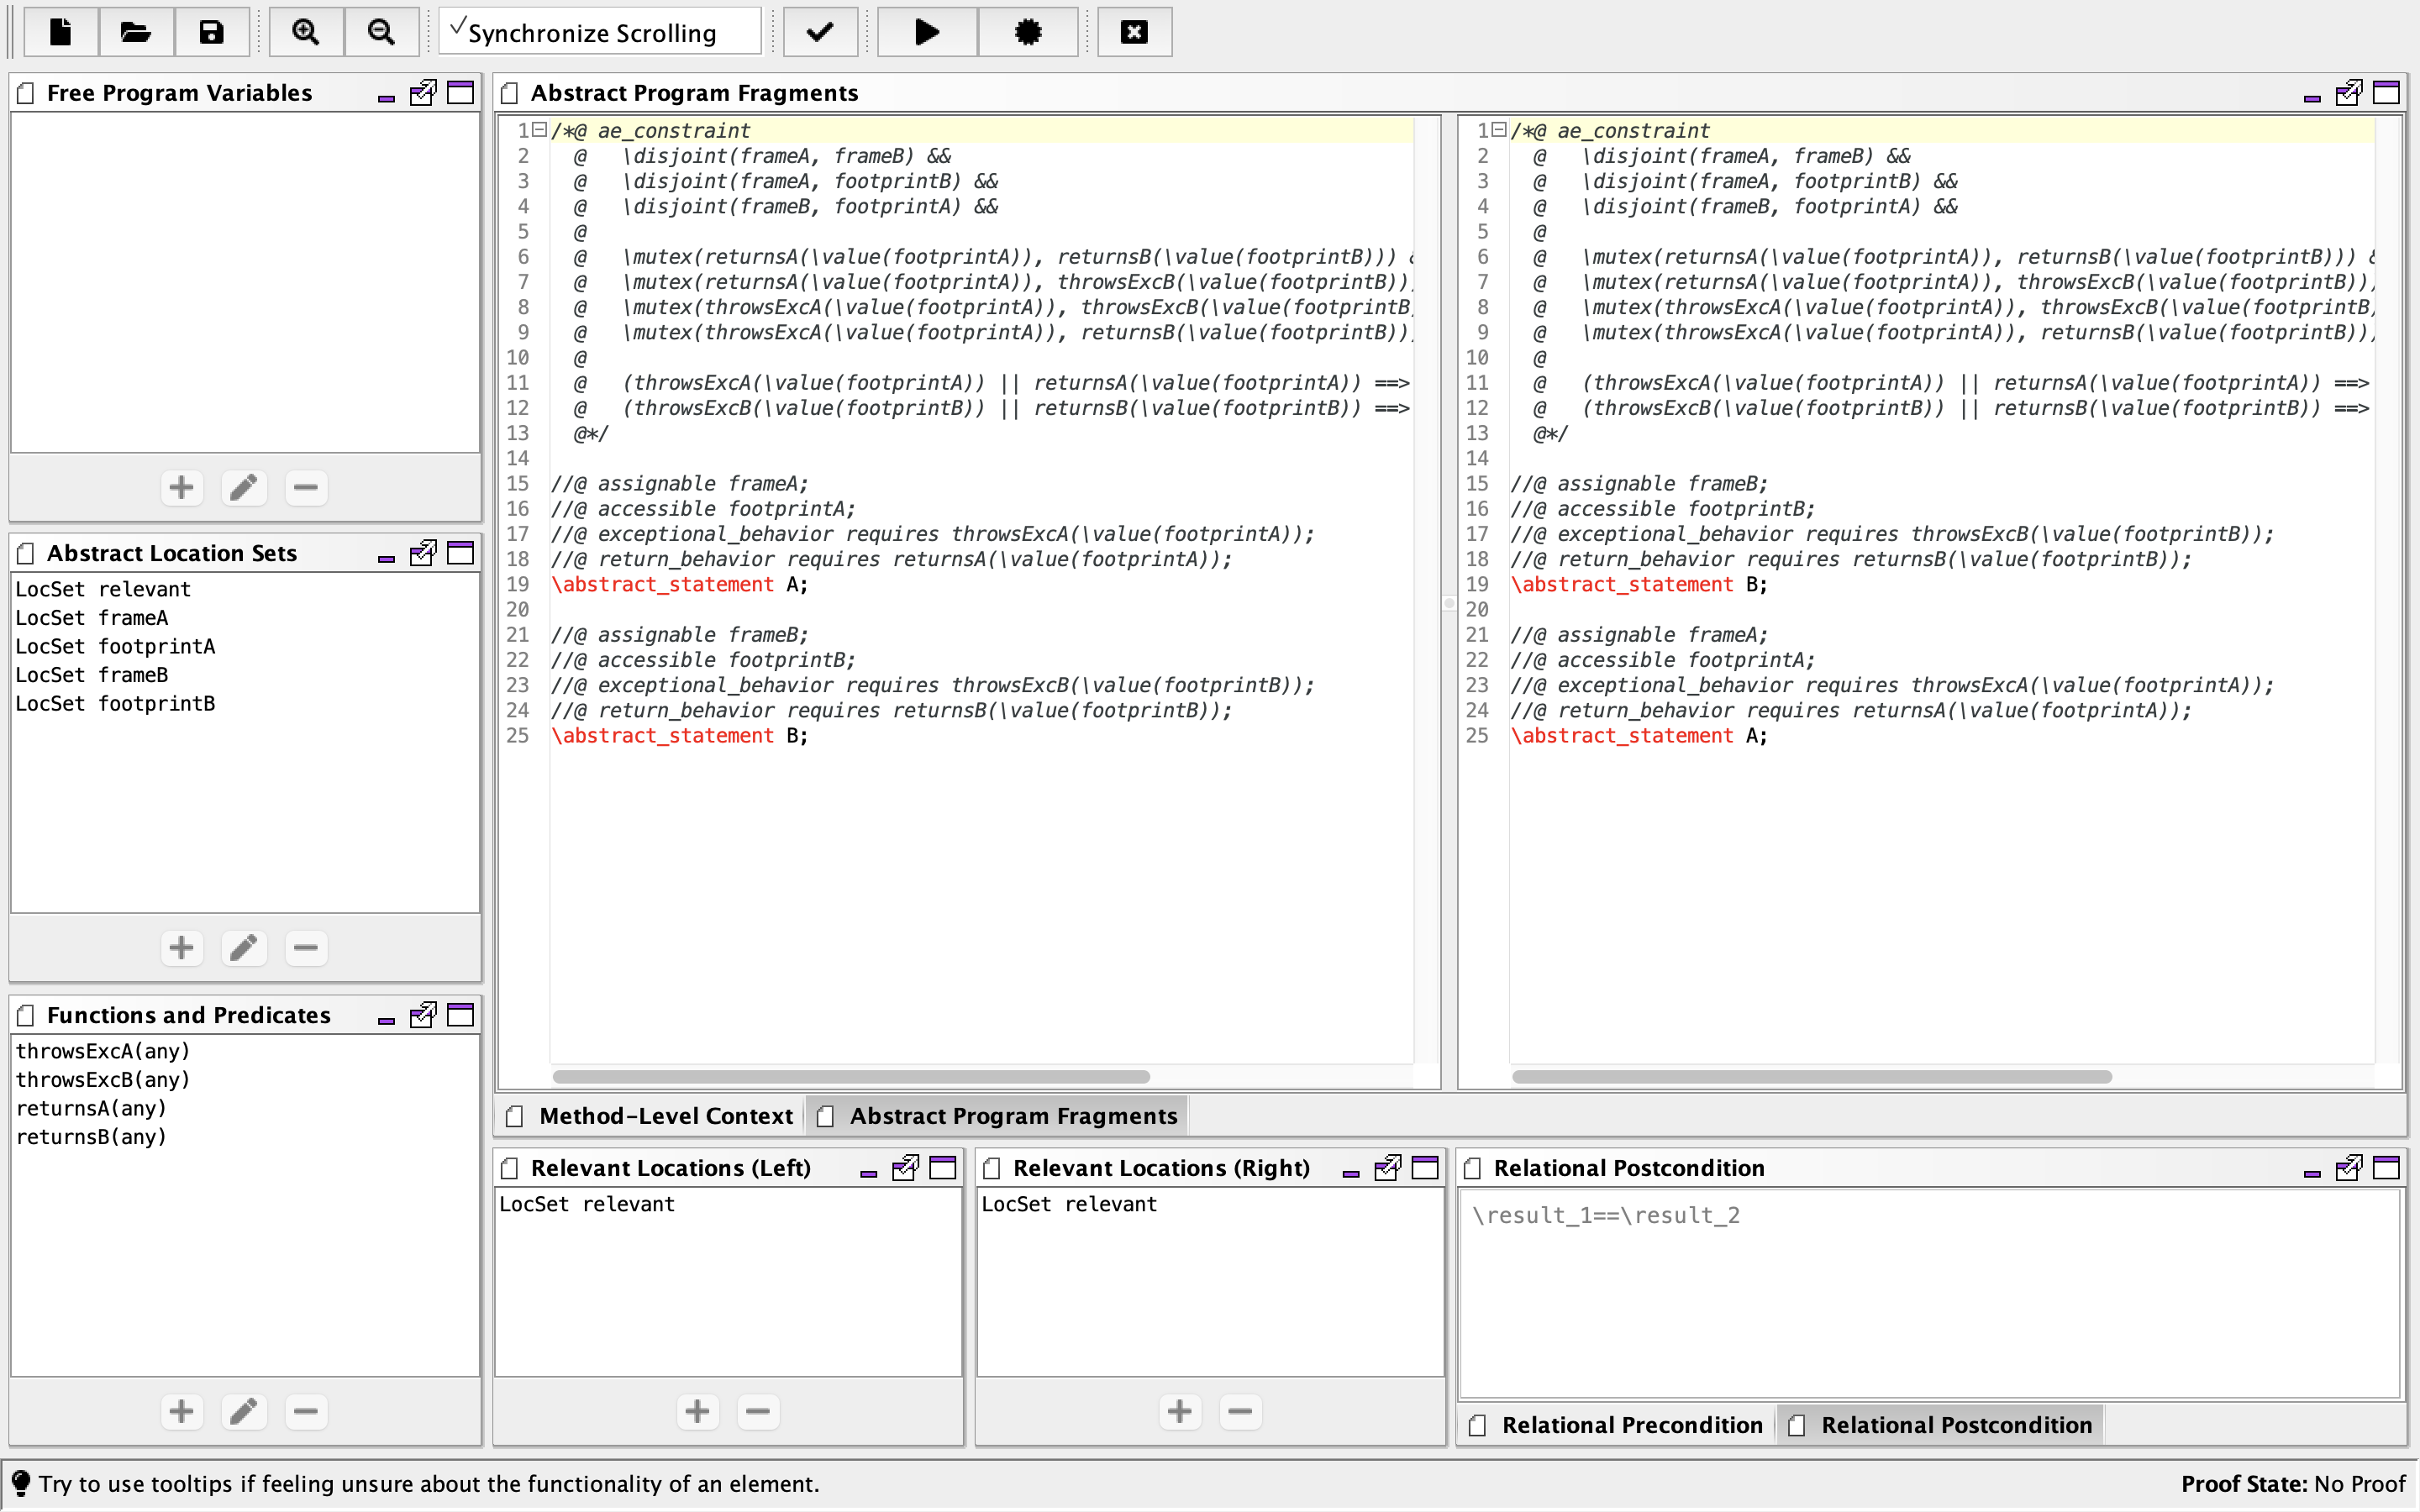
\includegraphics[scale=.25]{screenshots/SlideAbstract}
  \end{center}    
\end{frame}

\nexthint{Example - slide stm. concrete}
\begin{frame}\vspace*{-5mm}
  \begin{center}
    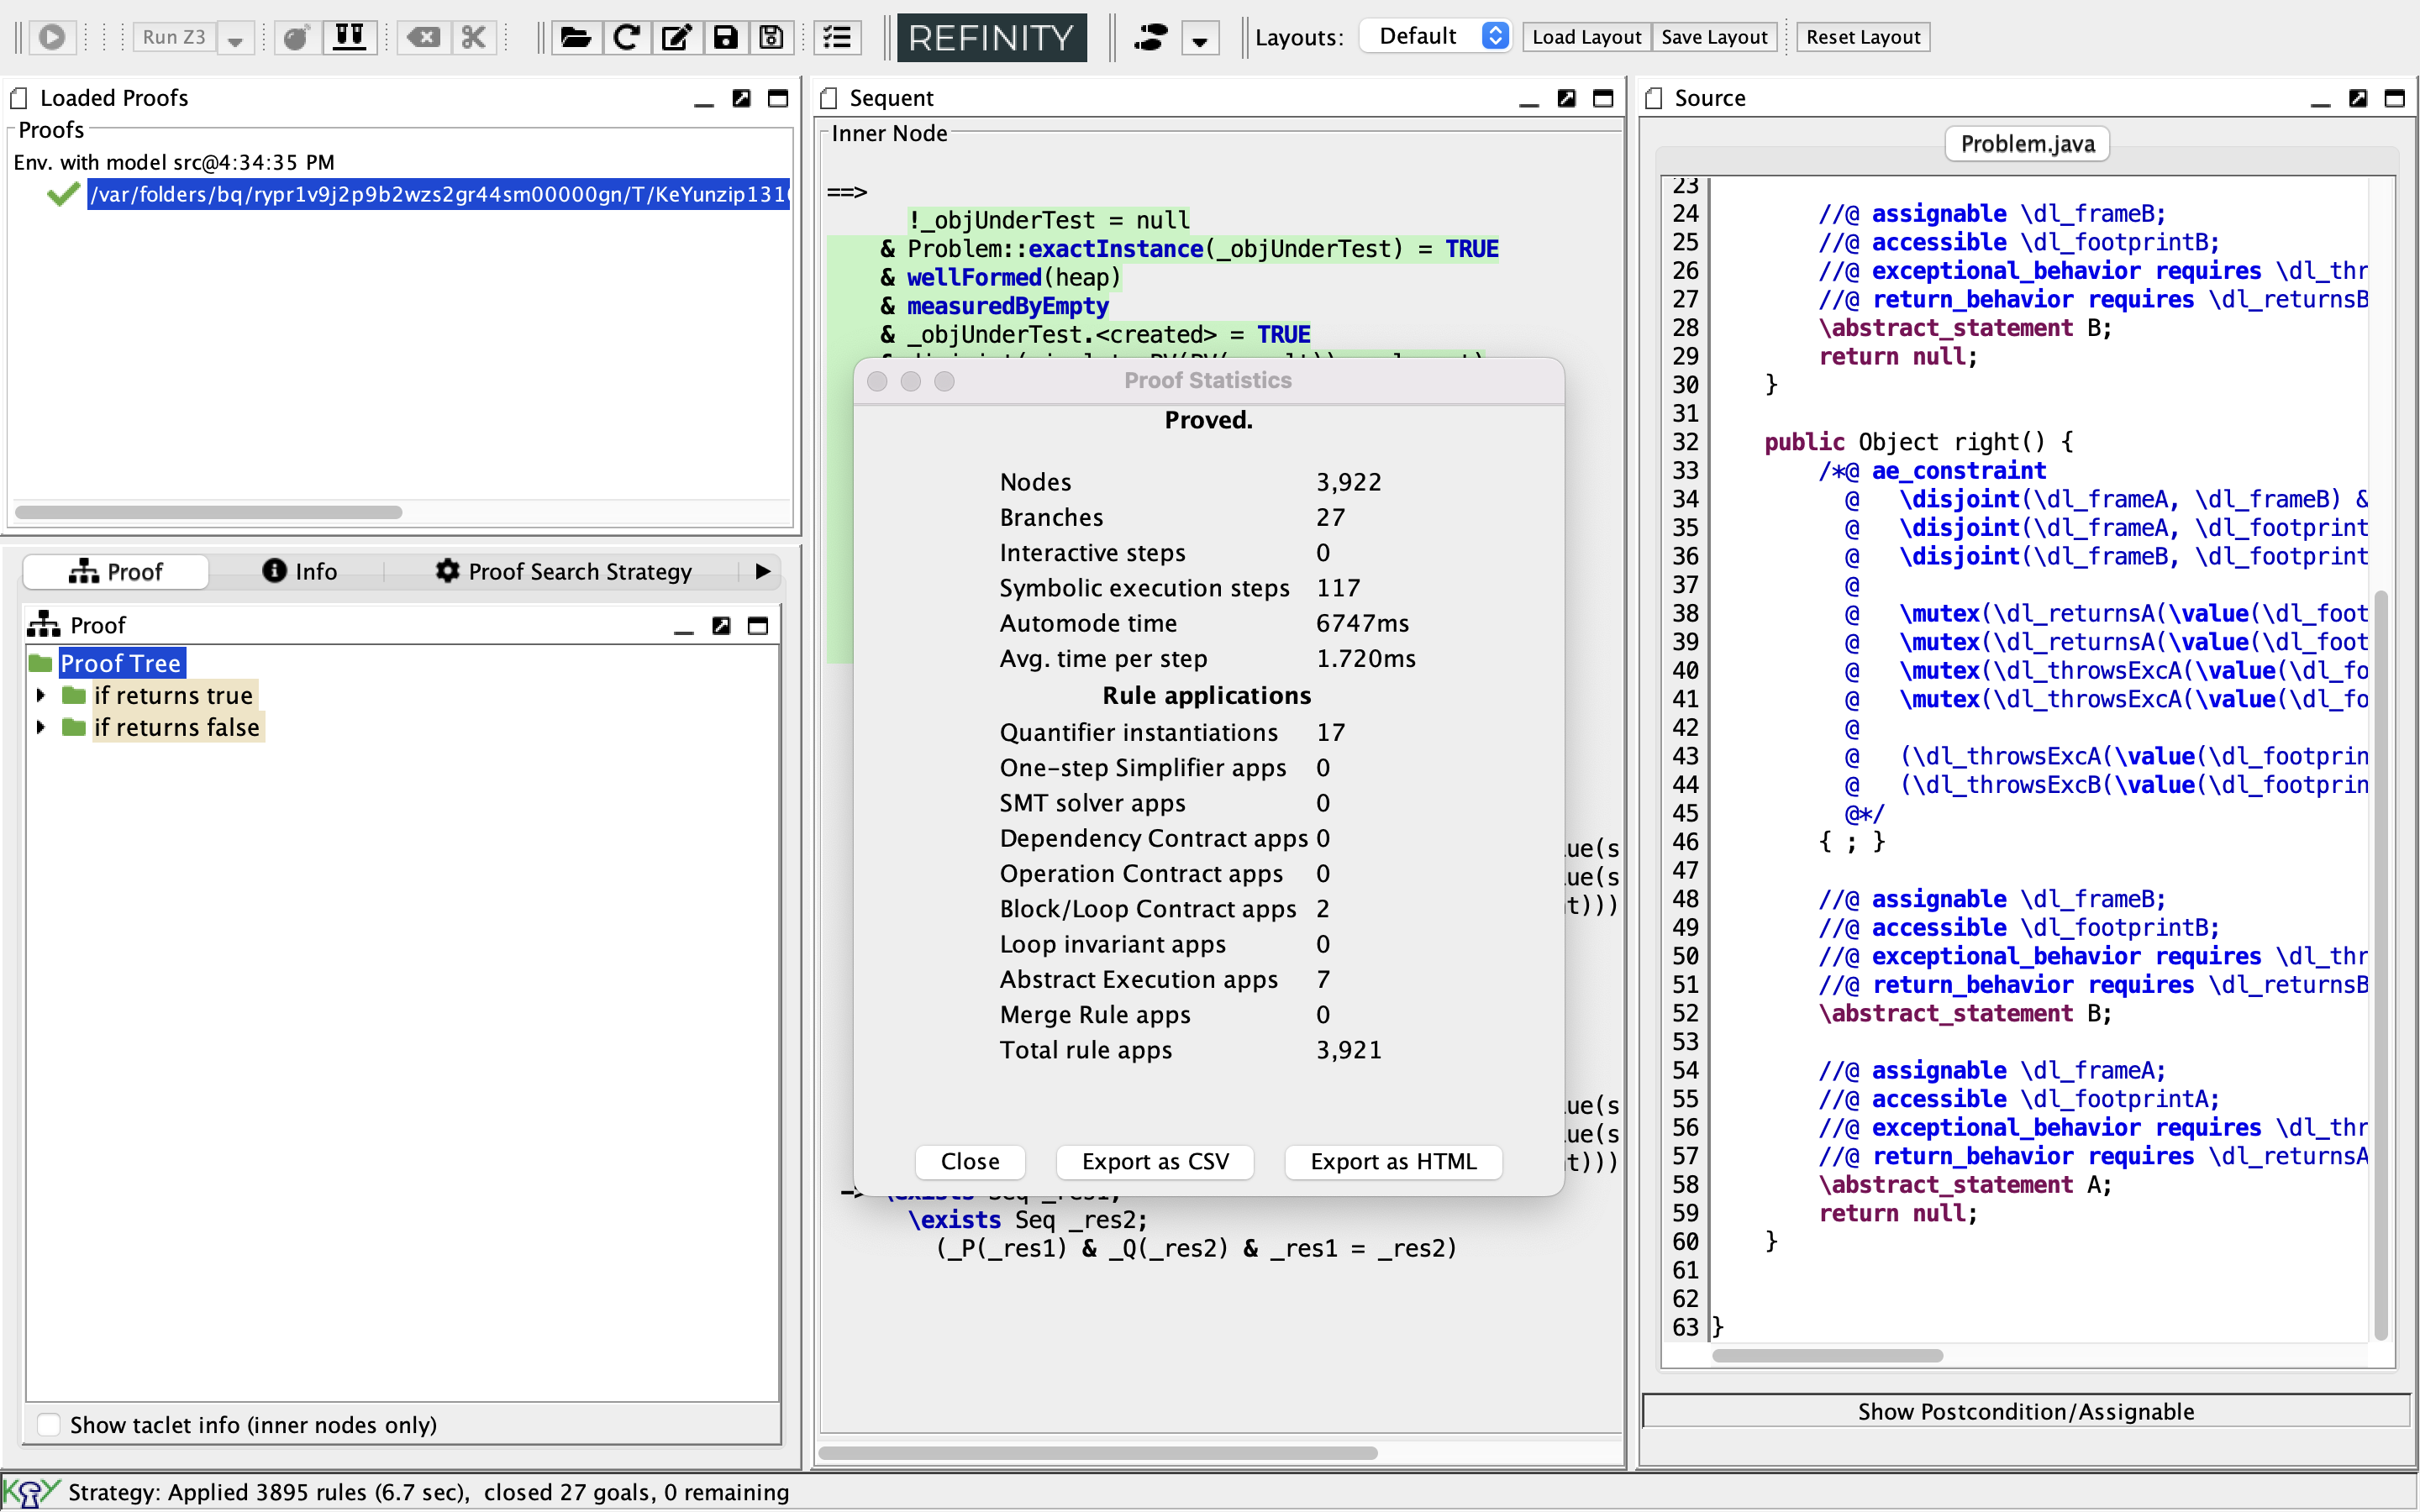
\includegraphics[scale=.25]{screenshots/SlideAbstractProved}
  \end{center}    
\end{frame}

\nexthint{Example - slide stm. conc. open goal}
\begin{frame}\vspace*{-5mm}
  \begin{center}
    \includegraphics[scale=.25]{screenshots/Slide}
  \end{center}    
\end{frame}

\nexthint{Equivalence in REFINITY}
\begin{frame}\vspace*{-5mm}
  \begin{center}
    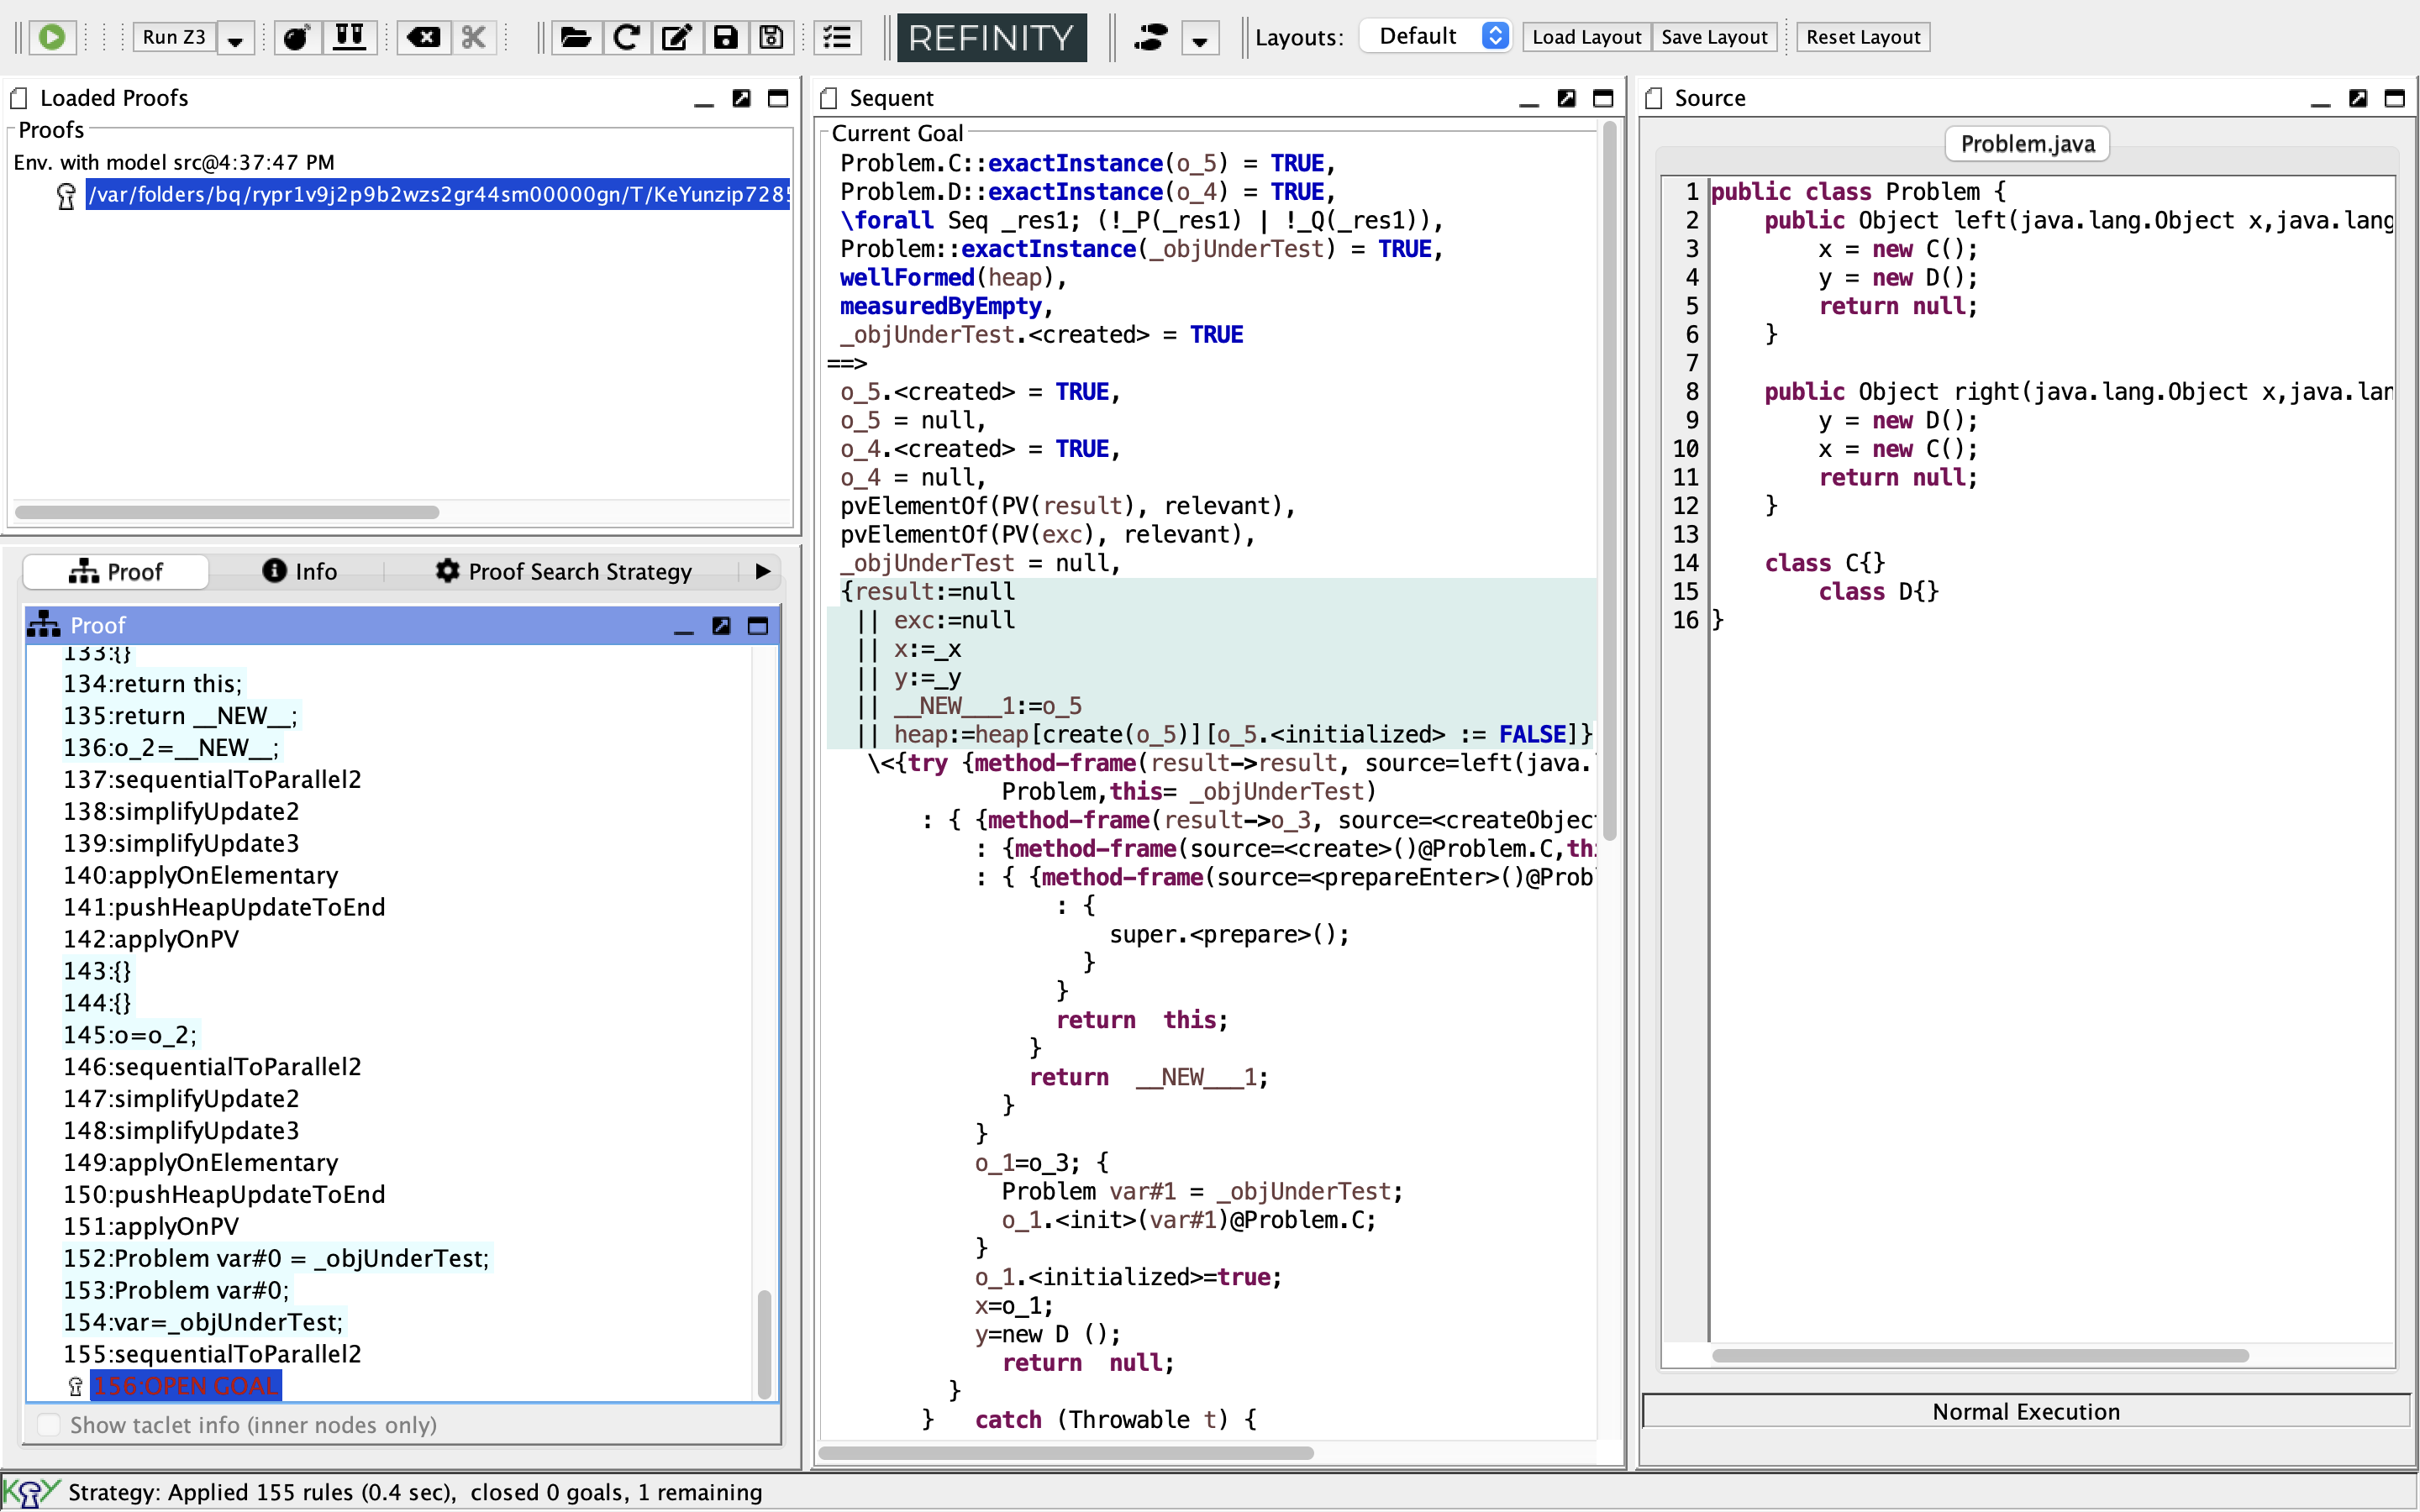
\includegraphics[scale=.25]{screenshots/SlideFail}
  \end{center}    
\end{frame}

\nexthint{Extract Local Variable}
\begin{frame}{Equivalence}
  REFINITY checks that the following are identical by default:
  
  \begin{itemize}
   \item return values
   \item exceptions
   \item objects in the so-called relevant location set
  \end{itemize}
\end{frame}




\nexthint{Example - condition on \lstinline[basicstyle=\tiny]{n()} in REFINITY}
\begin{frame}{Equivalent?}
  Refactoring tools often get this wrong:

\nexthint{Hide Delegate}
\begin{center}
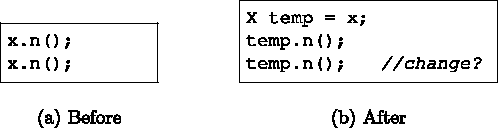
\includegraphics[scale=1.2]{imported/Listing2}
\end{center}

  REFINITY won't close the proof unless you can show the required
  side-conditions on method \lstinline{n()}.

\end{frame}

\nexthint{Hide Delegate}
\begin{frame}\vspace*{-5mm}
  \begin{center}
    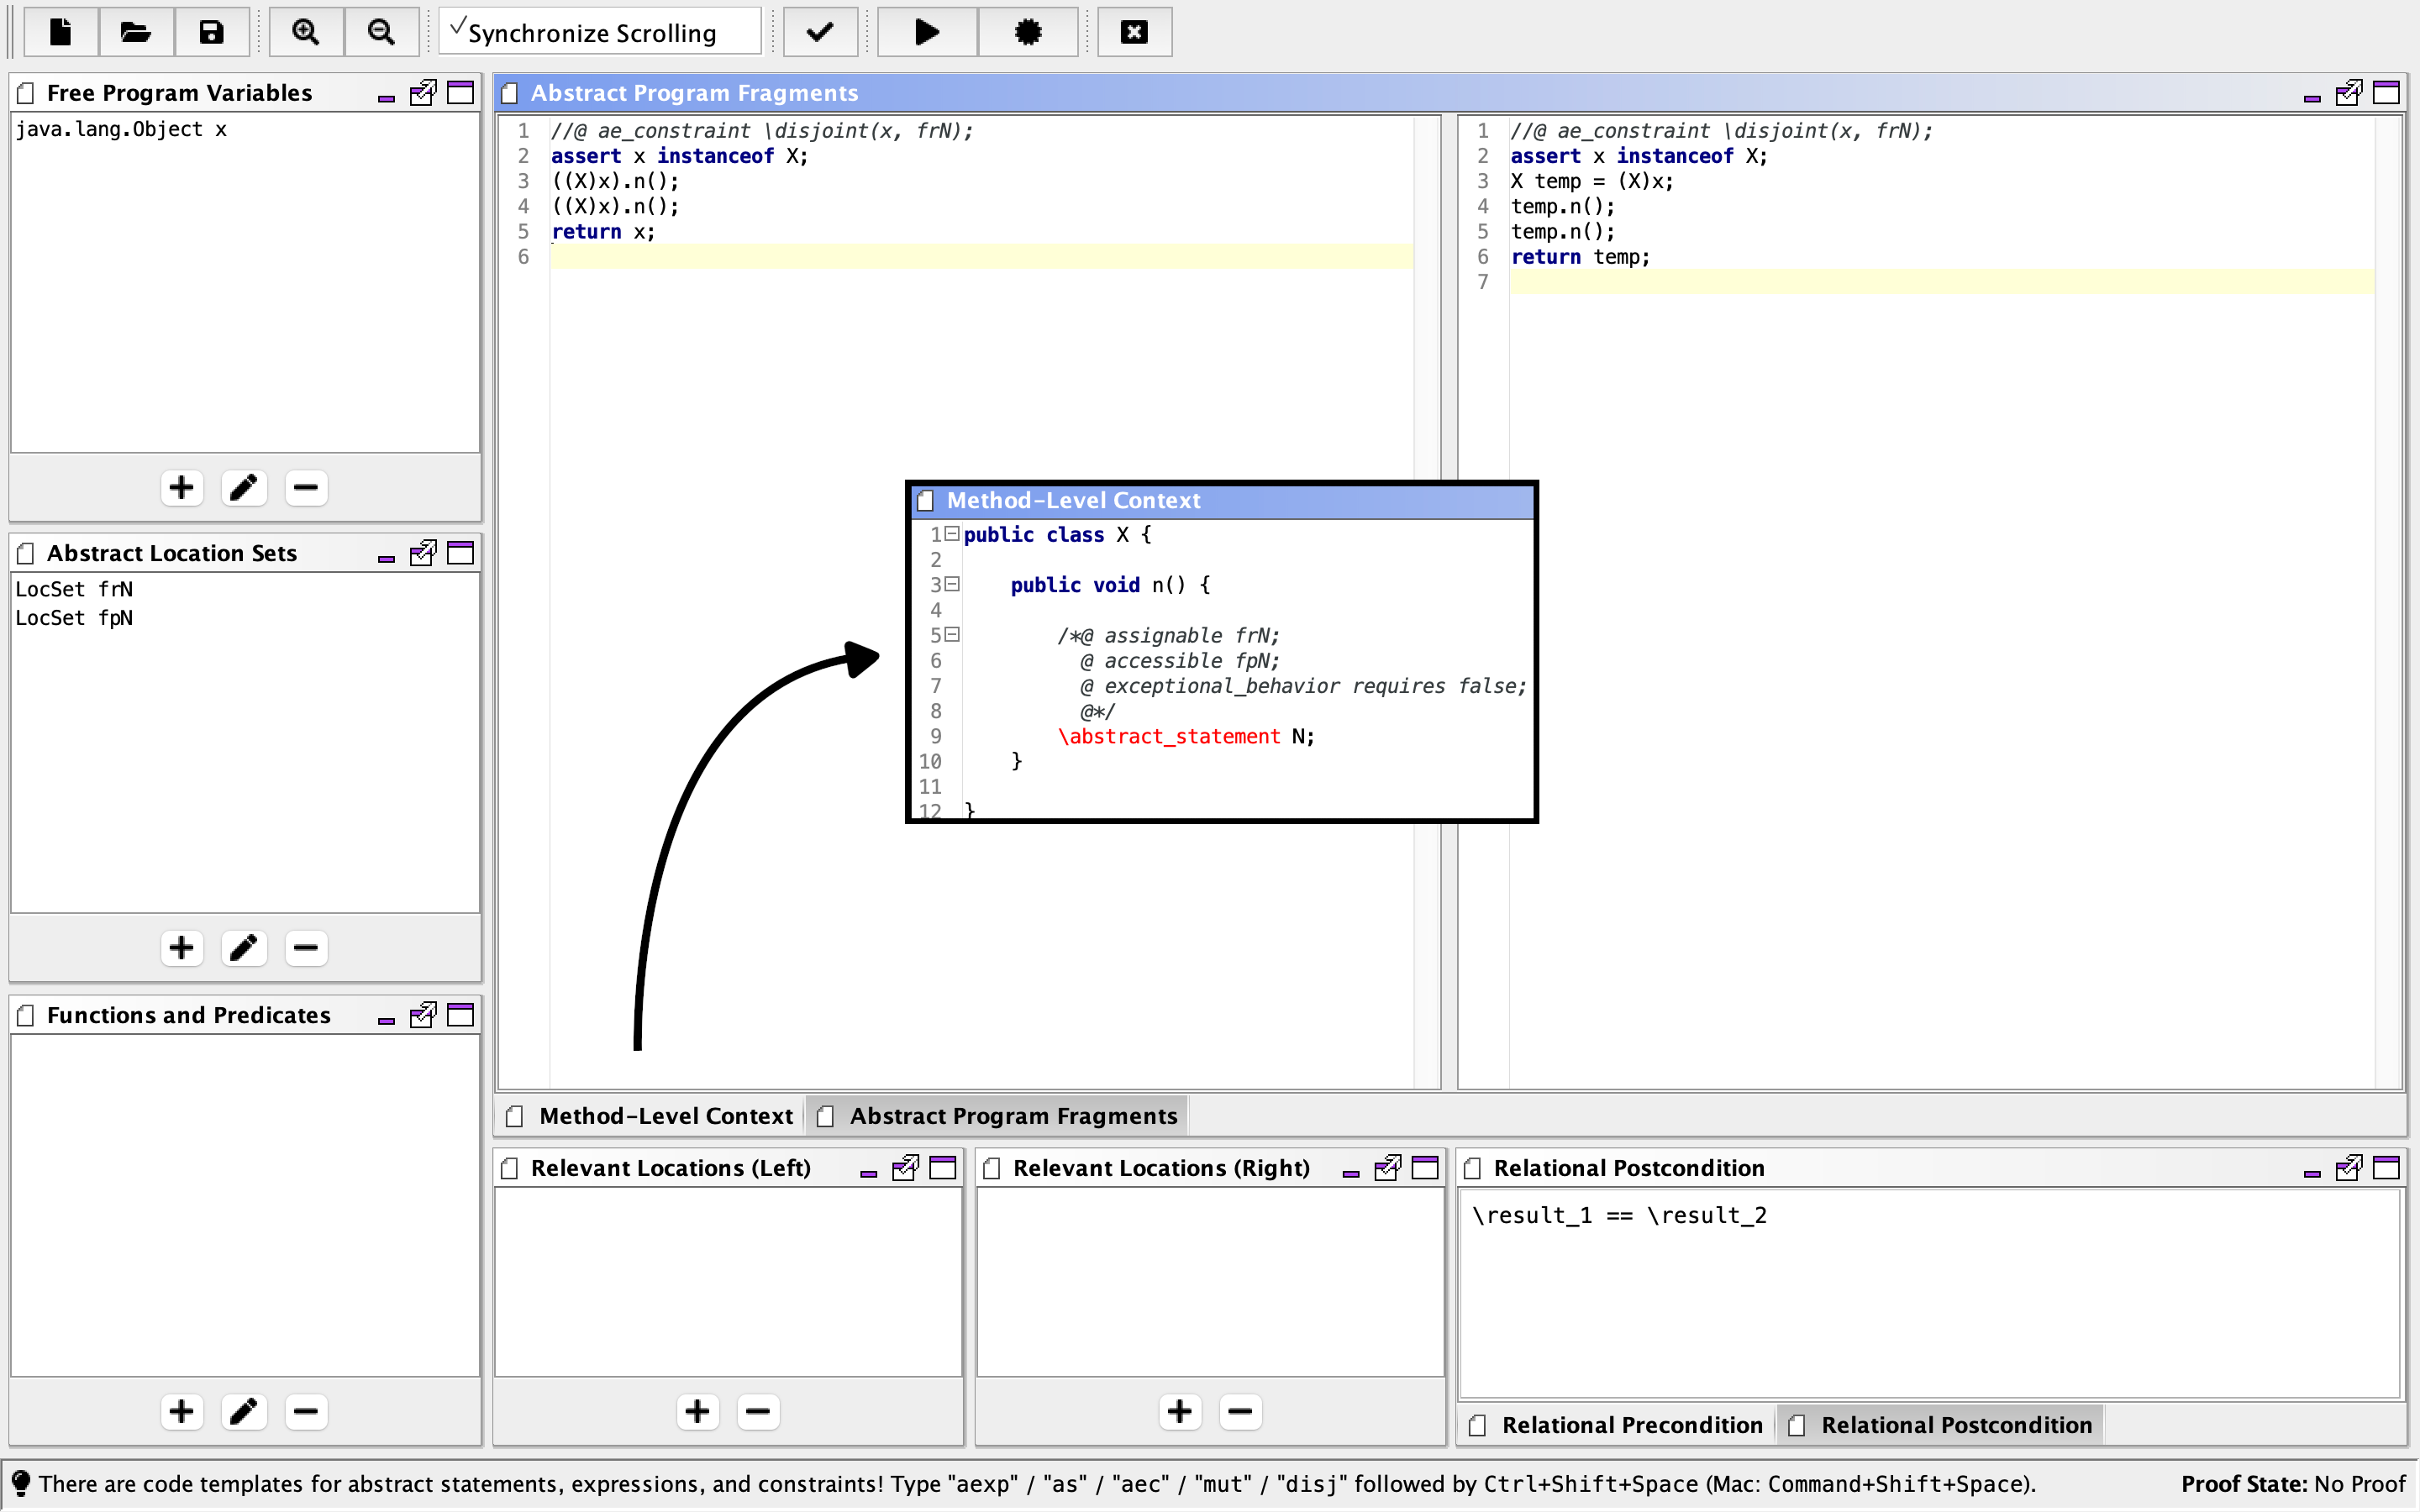
\includegraphics[scale=.25]{screenshots/ExtractLocalVariable}
  \end{center}   
\end{frame}


% \begin{frame}
% \begin{center}
% 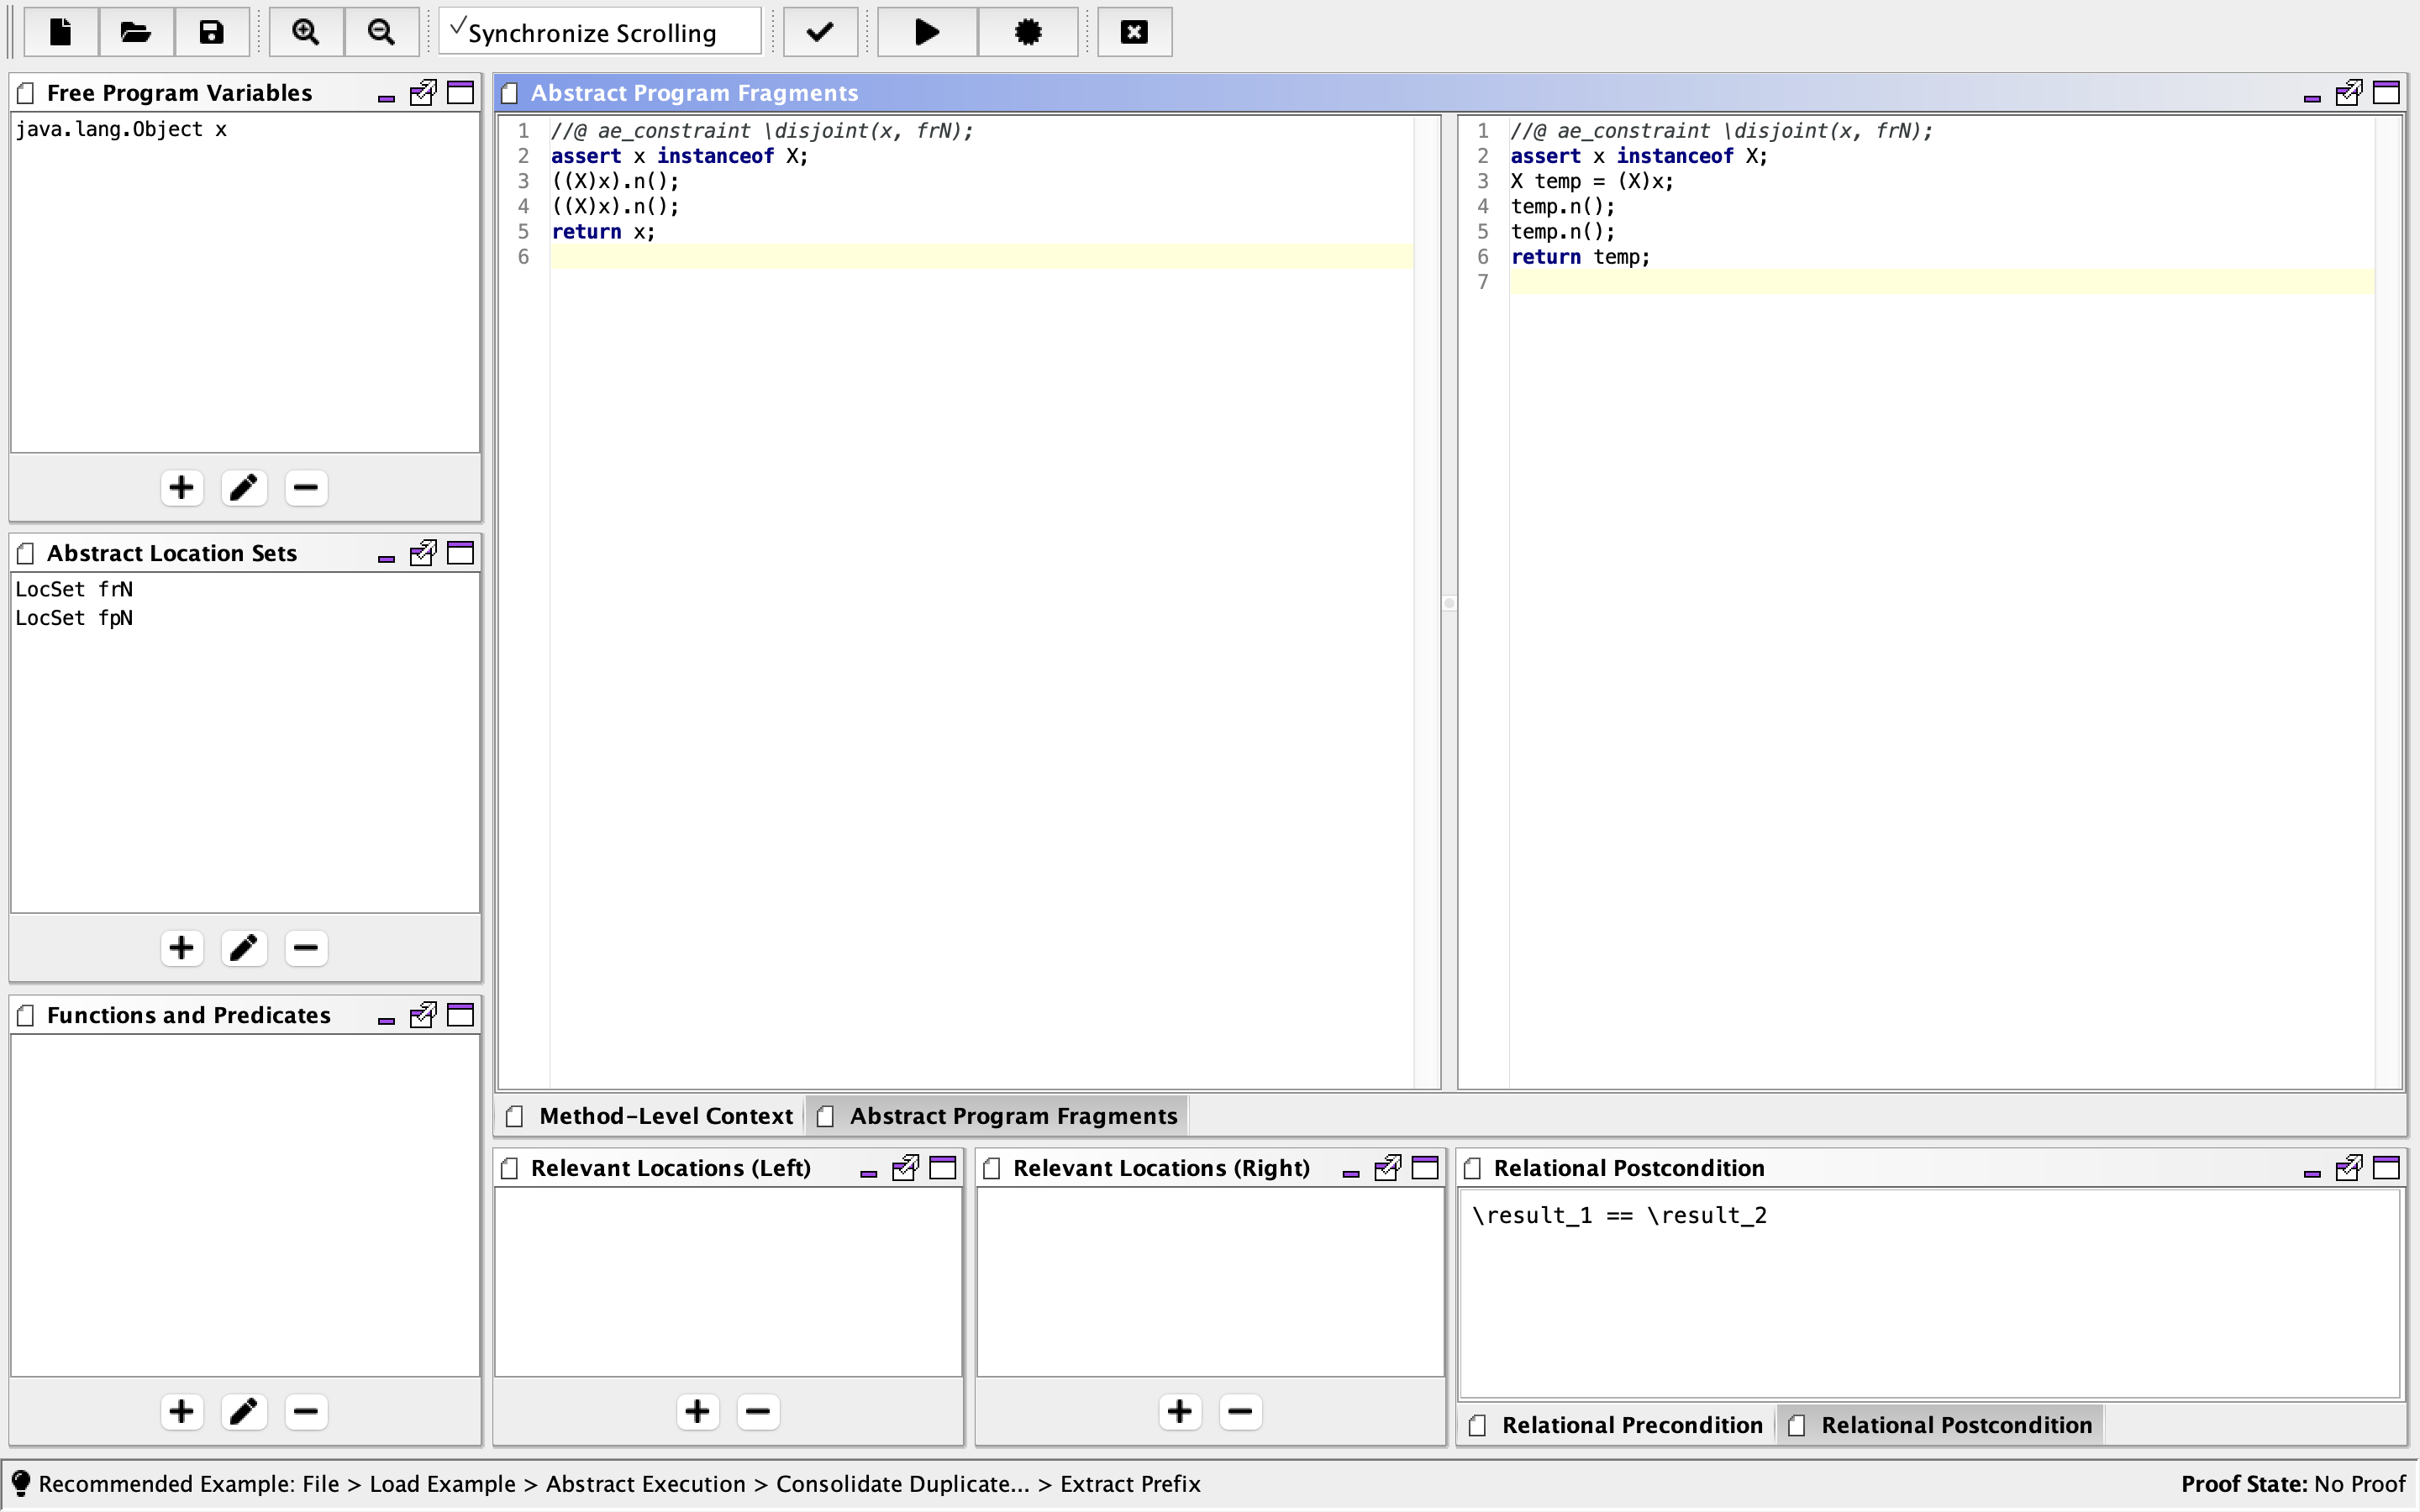
\includegraphics[scale=.26]{screenshots/ExtractVariableAbstract}
% \end{center}  
% \end{frame}

\nexthint{Example - in REFINITY (postcondition)}
\begin{frame}{Different output, but equivalent?}
Exception origin moved, no additional capture in \lstinline{h()}
\vspace{5mm}  
\begin{center}
  \begin{tabular}{rll}
    & \lstinline{o.f().g();}& \\
    $\rightarrow$ & \lstinline{o.h();} & with \lstinline{h()\{ this.f().g();\}}
  \end{tabular}
%{\small \texttt{o.f().g();} $\rightarrow$ \texttt{o.h(); $\mid$ h()\{ this.f().g(); \}}}
\end{center}
\vspace{1mm}       
\begin{minipage}{.49\textwidth}
\begin{figure}
  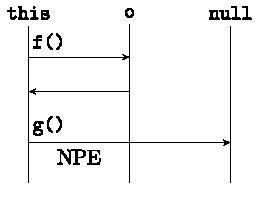
\includegraphics{imported/npe-before}
  \vspace{-1cm}
  \caption{original}
\end{figure}
\end{minipage}
\begin{minipage}{.49\textwidth}
\begin{figure}
  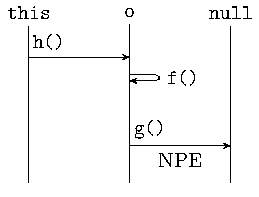
\includegraphics{imported/npe-after}
  \vspace{-1cm}
  \caption{refactored}
\end{figure}
\end{minipage}
\end{frame}

\nexthint{Challenges}
\begin{frame}\vspace*{-5mm}
\begin{center}
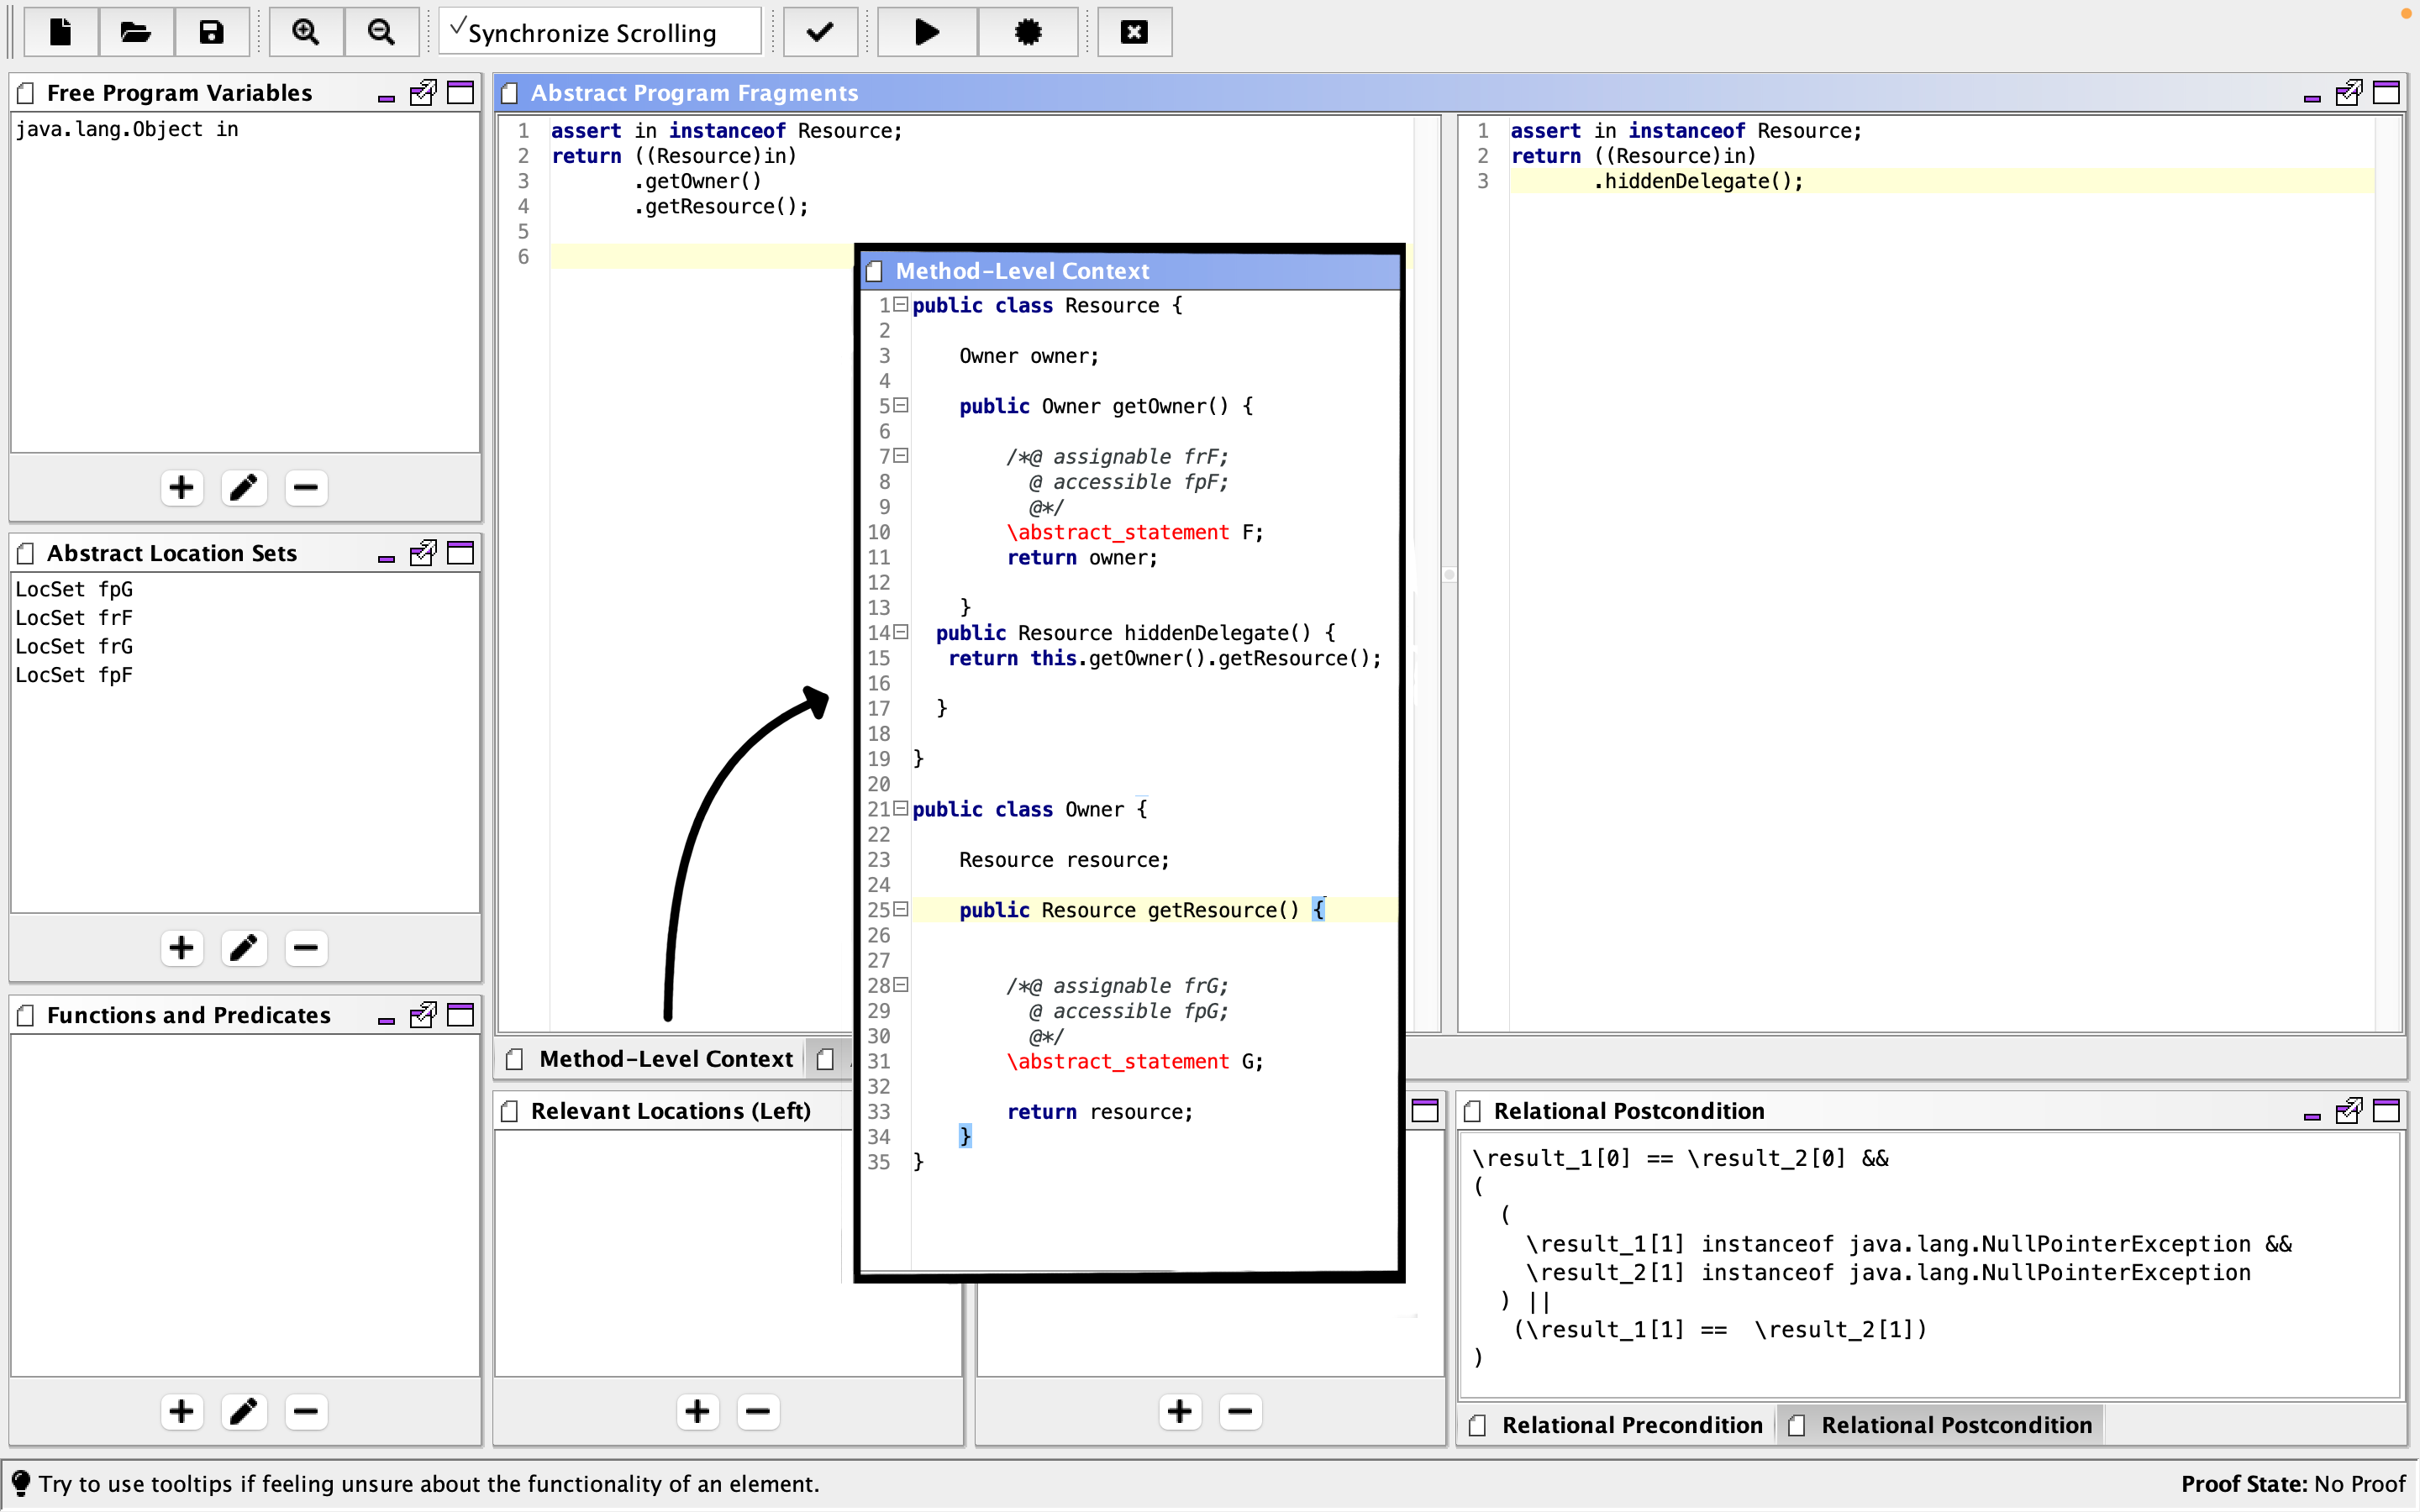
\includegraphics[scale=.25]{screenshots/HideDelegateAbstract}
\end{center}
\end{frame}

\nexthint{Object equality I}
\begin{frame}{Challenges in complex refactorings}
  Succesfully verified variants of \textit{Extract Local Variable} and \textit{Hide Delegate} and investigated how to approach others.
  \begin{block}{We discuss}
  Simplifying postcondition specifications
  \end{block}
  \begin{block}{Unresolved}
    Making the proofs useful artefacts:\\
    what about \emph{instantitations}?
  \end{block}
\end{frame}

